\documentclass[11pt]{article}
\usepackage[utf8]{inputenc}
\usepackage[top=60pt, bottom=60pt, left=70pt, right=70pt]{geometry}
\usepackage{graphicx,amsmath}
% Default fixed font does not support bold face
\DeclareFixedFont{\ttb}{T1}{txtt}{bx}{n}{8} % for bold
\DeclareFixedFont{\ttm}{T1}{txtt}{m}{n}{8}  % for normal
% Custom colors
\usepackage{color}

\definecolor{deepblue}{rgb}{0,0,0.5}
\definecolor{deepred}{rgb}{0.6,0,0}
\definecolor{deepgreen}{rgb}{0,0.5,0}
\definecolor{commentgrey}{rgb}{0.5,0.5,0.5}
\usepackage{listings}

\title{Computing the sunlit fraction}
\author{Daniel W. Zaide}
\date{\today}
\begin{document}
\maketitle
\section{Problem Statement}
Consider a set of rectangular facades, $S$, such as in Figure \ref{geomex}. We assume they form a fairly convex shape (they don't point towards eachother). 

\begin{figure}[!ht]
\centering
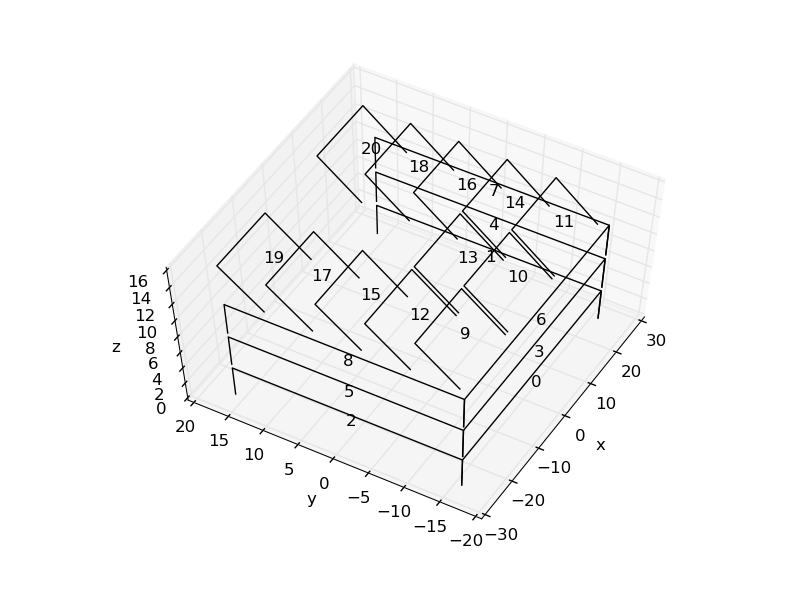
\includegraphics[width=0.6\textwidth]{images/whole-building.png}
\caption{Example geometric layout.}
\label{geomex}
\end{figure}
A facade is initially defined by its four coordinates, $\mathbf{p}_{0}, \mathbf{p}_{1}, \mathbf{p}_{2},\mathbf{p}_{3}$. The coordinates are provided in counter clockwise order, starting from the bottom left as in Figure \ref{definitions}. We can compute the outward normal vector from the first three points
\[
\mathbf{n} = (\mathbf{p}_2-\mathbf{p}_0) \times (\mathbf{p}_1-\mathbf{p}_0)
\] and further define the orientation and tilt angles as
\[
\theta_{\mathrm{orient}} = 90+\tan^{-1}(\mathbf{n}_y/\mathbf{n}_x), 
\qquad \theta_{\mathrm{tilt}} = 90 - \tan^{-1}\left(\sqrt{\mathbf{n}_{x}^2+\mathbf{n}_{y}^2}/\mathbf{n}_z\right), 
\]

\begin{figure}[!ht]
\centering
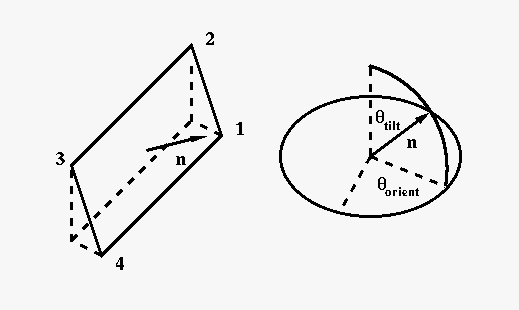
\includegraphics[width=0.50\textwidth]{images/geomdefine.png}

\caption{Facade definitions}
\label{definitions}
\end{figure}
The problem statement is then, {\bf
Given the set of facades and a sun vector, determine the fraction of each facade shaded by every other facade.} The idea is to first precompute a list of other facades for each facade that could shade it, and thus, minimize the amount of work that has to be done for a particular sun vector at each time, such that each facade does not need to be checked against every other facade for every sun vector.

\section{Determining which facades \emph{can} shade another}.
We first begin by determining which facades could potentially shade another. Given a facade, $s \in S$ with coordinates $\mathbf{s}$, call the subset of $S$ that can potentially shade, $R \subset S$. $R$ does not include any facade that can never shade it, for all potential sun locations.  Any facade $r$ that could shade $s$, must have at least (in approximate order of ease of computation)
\begin{enumerate}
\item $\mathbf{n}_{s}\cdot \mathbf{n}_{r} > 0$, their normals must point in the same general direction.
\item $\min(\mathbf{s}_{z}) < \max(\mathbf{r}_{z})$, $r$ cannot be completely below $s$
\item $(\mathbf{r}_i-\mathbf{s}_i) \cdot \mathbf{n}_s > 0, i = 0,1,2,3$, $r$ must have at least one point "in front" of $s$ \footnote{This is the condition I'm least certain about how strongly I need to enforce, and I believe that the requirement is simply that one point in $r$ is in front of the plane of $s$, which can be checked in a number of ways, but there are a minimum of four comparisons.}
\end{enumerate}
$R$ is then constructed to consist of $r$ that satisfies this set. The last check for the subset $R$ is whether any $r$ is completely blocked by the other facades in the subset, $q$, in which case, it does not need to be in the subset. This can be checked by projecting $r$ through each $q$ onto $s$, to see if $q$ partially blocks $r$. After checking all $q$, if $r$ is completely blocked, it is removed from the set $R$. This is done using the overall shading algorithm, described in the next section. Every facade left in $R$ can now potentially shade $s$.

For the example in Figure \ref{geomex}, the subsets are as follows
\begin{verbatim}
0 has subset [3], 1 has subset [4], 2 has subset [5], 
3 has subset [6], 4 has subset [7], 5 has subset [8]
12, 13, 14 have subsets [9, 10, 11]
15, 16 have subsets [10, 12, 13, 14]
17 has subset [11, 13, 14, 15, 16]
18 has subset [9, 12, 13, 15, 16]
19 has subset [11, 13, 14, 16, 17, 18]
20 has subset [9, 12, 13, 15, 17, 18]
\end{verbatim}
where there is additional information potentially available from this last stage, for example, for facade 20, facade 9 can shade at most 5\% of it (through the gap), facade 12 can shade at most 40\% of it and facade 13 can shade at most 35\% of it.

\section{Calculating the sunlit fraction at a particular sun location}
We begin with a vector corresponding to the sun, given at a specific time, $\mathbf{n}_{sun}(t)$, pointing inward towards the facades. We know it points downward at all times, 
\[
  \mathbf{n}_{sun,z}(t) \leq 0
\]
which is used in the above section to form the subset. This vector is the negative of the vector given from the solar azimuth and altitude. Given a facade, $s$, and its subset of all facades, $R$, the fraction not shaded (sunlit fraction) can be determined, denoted by $\eta \in [0,1]$. We note that the sunlit fraction is 0 if the sun does not see $s$,
\[ \mathbf{n}_{sun}\cdot \mathbf{n}_s  > 0\]

If the sun can see $s$, first, consider the projection of $r$ onto $s$. 
The coordinates of this projection, $r_{s}$ are calculated as $\mathbf{r}_{s,i} = \mathbf{r}_i+p_i\mathbf{n}_{sun}$, where $p_i$ is a parameter obtained by solving for the intersection of the ray and the plane, given by
\[
p_i = \frac{\mathbf{n}_s\cdot (\mathbf{s}_0-\mathbf{r}_i)}{\mathbf{n}_s\cdot \mathbf{n}_{sun}}
\]
where the plane is defined by its normal and a point on it, in this case, $\mathbf{s}_0$. From our creation of the subset, at least one $p_i > 0$, ensuring there is some sight line from $r$ to $s$ along $\mathbf{n}_{sun}$. We now have two surfaces lying on the plane of $s$. Denote the intersection of $s$ and $r_{s}$ as $s \cap r_{s}$, the shaded area. The sunlit component is $s-(s \cap r_{s})$ and the sunlit fraction of $s$ due to $r$, $\eta_{s,r}$
\[
\eta_{s,r} = \frac{s-(s \cap r_{s})}{s} = \frac{\text{area of s - area shaded}}{\text{area of s}}
\]
Thus if the intersection is empty, there is no shading, and if the intersection is $s$, the facade is fully shaded. To compute $s \cap r_{s}$, we project both to a neutral frame in $\mathbf{R}^2$, the $x-z$ plane, by rotating first about the orientation and then about the tilt angle, using rotation matrices\footnote{If we did not do this projection step, and attempted to solve the intersection of two polygons on an arbitrary plane in $\mathbf{R}^3$, numerical precision would almost guarantee that none of their edges would ever exactly intersect.}. With this projection completed, an external library can be used to determine the intersection\footnote{Computing the intersection between polygons is non-trivial, and such, an external package is used.}. The total sunlit fraction of $s$ is determined by solving this problem for all $r \in R$, and a final equation is
\[
\eta_{s} = \frac{s-(s \cap r_{0}\cap r_{1} \cap r_{2} \cap \ldots) }{s}
\]
which involves successively reducing the sunlit area with each possible facade's contribution. This is the same methodology used in the last step of determining $R$. Note that if the actual sunlit part of $s$ was required, a rotation back to its original plane would be needed, however, since we are interested a fraction, all of the work is done in the $x-z$ plane.

In summary, the algorithm is as follows for facade $s$

\begin{itemize}
\item For each facade $r \in R_s$:
\item \hspace{0.5cm} Project $r$ onto $s$ along $\mathbf{n}_{sun}$ to get $r_s$.
\item \hspace{0.5cm} Rotate both $r_s$ and $s$ by their tilt and orientation onto the $x-z$ plane
\item \hspace{0.5cm} Calculate the sunlit part of this projection in the $x-z$ plane, $s-(s \cap r_{s})$
\item Finally, calculate the sunlit fraction by calculating the total sunlit area, $s-(s \cap r_{0}\cap r_{1} \cap r_{2} \cap \ldots)$, working entirely in the $x-z$ plane.
\end{itemize}

Consider our simulations, with a time $t_i$ and timestep $\Delta t$. The sunlit fraction at any time is 
\[ 
\eta_{s}(t_i) = \frac{s-(s \cap r_{0}(t_i)\cap r_{1}(t_i) \cap r_{2}(t_i) \cap \ldots) }{s}
\]
In practice, we should use an averaged value,
\[ 
\eta_{s}(t_i) = \int_{t_i-\Delta t/2}^{t_i+\Delta t/2} \frac{s-(s \cap r_{0}(t)\cap r_{1}(t) \cap r_{2}(t) \cap \ldots) }{s} \mathrm{d}t
\]
which we can estimate by numerical integration, using any number of methods. This is implemented in geom.py as part of the GeometrySet object, which contains the subsets and other information. The averaging is computed in shading.py


\end{document}
